\documentclass{article}

\usepackage[UTF8]{ctex}
\usepackage{amsmath,amssymb}
\usepackage{geometry}
\usepackage{graphicx}

\geometry{a4paper, margin=2.5cm}

\begin{document}

% ============================================================
\section*{GRPO 与可验证奖励（RLVR / Reinforcement Learning with Verifiable Rewards）}

\subsection*{先讲一个故事}

前两章的所有麻烦都出自同一个源头：奖励是从有限覆盖的偏好数据里\textbf{学}出来的代理，代理与真实之间的缝隙会被优化器无限放大。但很多任务根本不需要学奖励——数学题的答案对不对，一条规则就能判；代码对不对，跑一遍测试就知道。

\textbf{错误做法 / 朴素做法}：给会判分的任务也训一个奖励模型。它会从数据里学到「看起来对」的特征，然后被优化器击穿——第 11 章的全部剧情重演一遍。

\textbf{本章方法的做法}：能验证就别学。用规则验证器直接给出奖励（对 $=1$、错 $=0$），配一个不需要 Critic 的策略梯度算法——GRPO：同一提示采样一组回答，用组内相对表现作为优势。

\textbf{本章的核心问题}：当奖励不可击穿之后，新的瓶颈是什么？

\[
\boxed{\hat{A}_{i} = \frac{r_{i} - \mathrm{mean}(r_{1},\dots,r_{G})}{\mathrm{std}(r_{1},\dots,r_{G})}}
\]

\subsection*{数学形式化}

对每个提示 $x$，从当前策略采样 $G$ 个补全 $\{y_{i}\}_{i=1}^{G}$，验证器给出奖励 $r_{i}=\mathrm{verify}(x, y_{i})\in\{0,1\}$。GRPO 的目标与 PPO 同构，但优势由组内标准化给出：

\[
\boxed{J(\theta) = \mathbb{E}\left[\frac{1}{G}\sum_{i=1}^{G} \min\!\left(\rho_{i}\hat{A}_{i},\; \mathrm{clip}(\rho_{i}, 1\!-\!\epsilon, 1\!+\!\epsilon)\,\hat{A}_{i}\right)\right]}
\]

\begin{itemize}
  \item $\mathrm{verify}$ —— 规则验证器：精确匹配、单元测试、约束检查，不含可学习参数；
  \item $G$ —— 组大小，同一提示的采样数，组内均值扮演该提示专属的基线；
  \item $\rho_{i}$ —— 新旧策略在补全 $y_{i}$ 上的概率比值，与第 7 章的 PPO-clip 相同；
  \item $\hat{A}_{i}$ —— 组相对优势：不需要价值网络，按提示难度自动归一。
\end{itemize}

% ============================================================
\section*{任务设计：让基础模型「自信地错」}

实验用两位数加法：提示为「d d + d d =」，补全 3 位数字，奖励为精确匹配。关键设计在 SFT 教师：它以 $0.3$ 的概率给出正确答案，以 $0.7$ 的概率给出\textbf{逐位相加不进位}的答案。于是在带进位的题目上，错误答案是数据的众数——基础模型贪心解码时进位准确率为 $0$，这不是噪声，是学进去的\textbf{系统性错误算法}。

这正是学习奖励无能为力的情形：奖励模型也从同一份有偏数据里学，只会把「不进位」学成高分特征。而规则验证器不看数据看答案：对就是对。GRPO 借助采样中残存的约三成正确率作为信号，约 20 轮把整体准确率从 $0.30$ 拉到 $1.00$，进位准确率从 $0$ 拉到 $1.00$（图~1）。

\begin{figure}[!htbp]
  \centering
  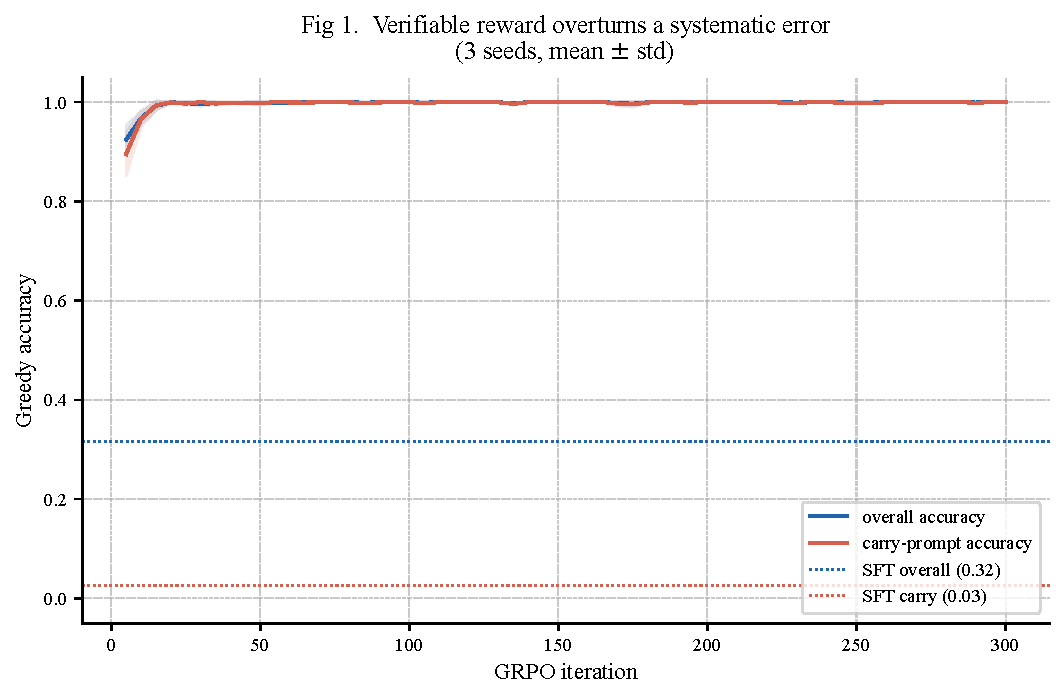
\includegraphics[width=0.88\textwidth]{fig1_rlvr_overturns.pdf}
  \caption{可验证奖励推翻系统性错误（两位数加法，3 个随机种子，阴影为 $\pm 1\sigma$，点虚线为 SFT 基线）。教师「不会进位」，SFT 基础模型整体准确率 $0.32$、进位题准确率 $0.03$；GRPO 约 20 轮把两者都拉到 $1.00$。}
  \label{fig:grpo-overturn}
\end{figure}

% ============================================================
\section*{核心机制}

\subsection*{机制一：不可击穿的奖励}

第 11 章里 $\beta=0$ 的 PPO 在 60 轮内击穿学习奖励；第 12 章里 DPO 的软锚随训练松动。这里同样 $\beta=0$、长训 600 轮：准确率到顶后纹丝不动，对参考策略的 KL 稳定在约 $1$ nat（图~2）。

原因不在算法在奖励：\textbf{验证器与真实目标是同一个函数}，代理与真实之间没有可分叉的缝隙，优化再狠也只能把正确答案学得更牢。KL 锚定从必需品变成可选项。剩下的风险只有一个——验证器本身有没有漏洞（答案格式绕过、测试用例不全），那是工程问题，不再是学习问题。

\begin{figure}[!htbp]
  \centering
  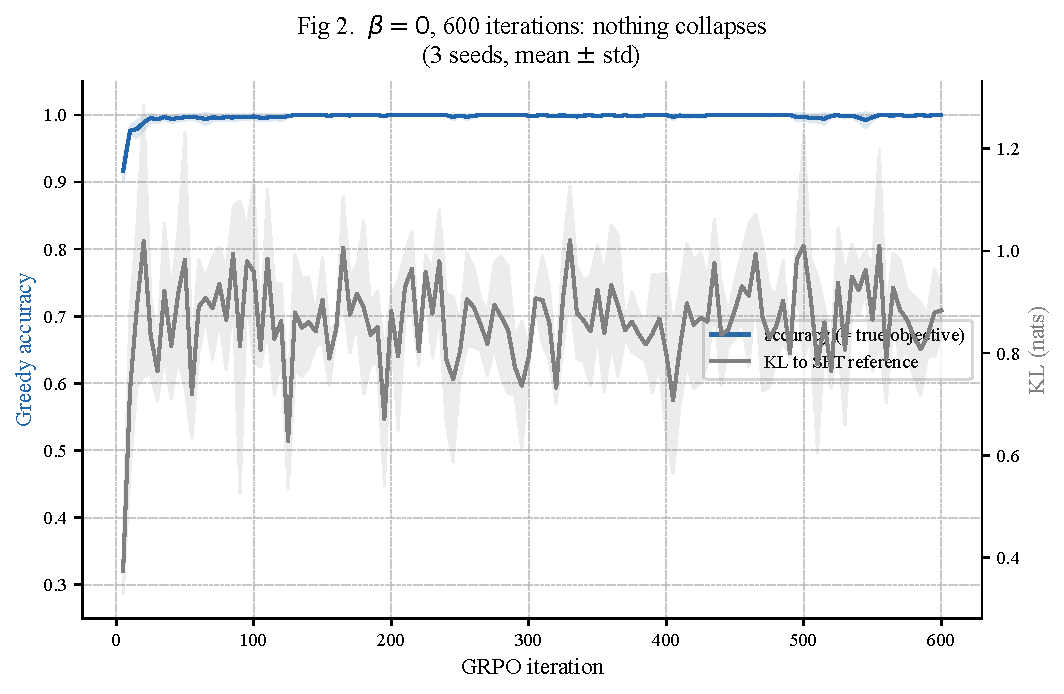
\includegraphics[width=0.88\textwidth]{fig2_unhackable_reward.pdf}
  \caption{$\beta=0$、600 轮长训（3 个随机种子，阴影为 $\pm 1\sigma$）。准确率（左轴）到顶后保持 $1.00$，KL（右轴）稳定在约 $1$ nat——对照第 11 章 $\beta=0$ 的崩塌与第 12 章的软锚松动：可验证奖励下无锚也不崩。}
  \label{fig:grpo-unhackable}
\end{figure}

\subsection*{机制二：组相对基线——用对比替代 Critic}

PPO 需要价值网络估计基线，GRPO 用「同一提示、一组回答」的组内均值替代：容易的提示组内全对、困难的提示组内全错，优势自动按提示难度归一，不需要任何额外网络。在本章的任务上，组基线与全局批基线表现相当——组机制的独特行为在下一个机制里显形。

\subsection*{机制三：零信号组——新的瓶颈是信号}

可验证奖励通常是稀疏的 0/1。组相对优势依赖\textbf{组内差异}：全对或全错的组标准差为零，优势恒为零，梯度恒为零。把教师换成从不给对进位题（$q=0$）：冷启动模型在进位题上采样成功率$\approx 0$，每个组要么全对（无进位题）要么全错（进位题），零信号组占比恒为 $100\%$——学习从未开始，准确率永远停在 $0.30$（图~3）。

同一个统计量在弱教师起点下讲另一个故事：零信号组占比从约三成升到接近 $100\%$，因为题目全部练会了——「毕业」。全组同分有两种含义，只有看着准确率才能分辨。这就是推理模型训练需要冷启动 SFT 数据与课程设计的原因：可验证奖励解决了「奖励可靠性」，把难题留给了「探索与信号密度」。

\begin{figure}[!htbp]
  \centering
  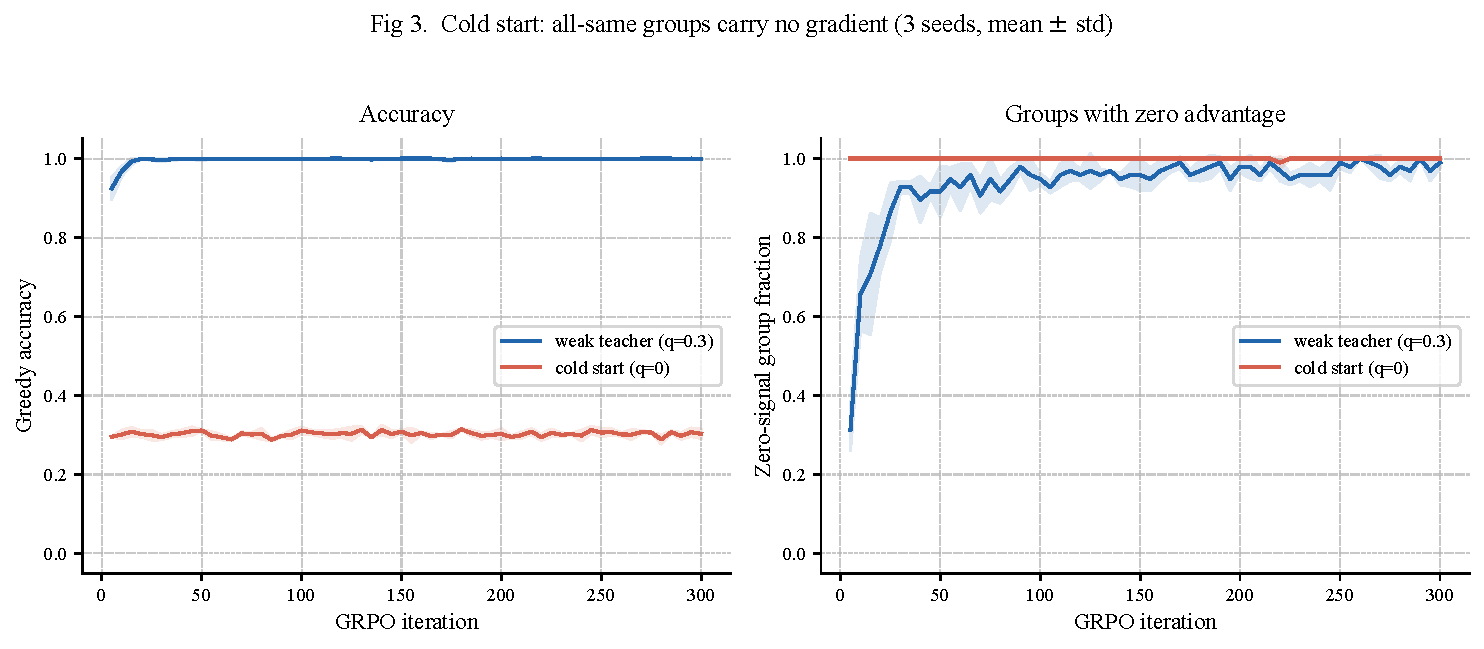
\includegraphics[width=0.88\textwidth]{fig3_cold_start.pdf}
  \caption{冷启动之死（3 个随机种子，阴影为 $\pm 1\sigma$）。左：弱教师起点（蓝）升到 $1.00$，冷启动（红，教师从不给对进位题）停在 $0.30$。右：零信号组占比——冷启动恒为 $100\%$（全组同分、零梯度），弱教师起点从约三成升到接近 $100\%$（题目练会、毕业）。}
  \label{fig:grpo-coldstart}
\end{figure}

% ============================================================
\section*{完整算法流程}

\subsection*{GRPO 一轮迭代}

\begin{enumerate}
  \item \textbf{采样}：取一批提示，每个提示从当前策略采样 $G$ 个补全；
  \item \textbf{验证}：规则验证器逐个打分 $r_{i}\in\{0,1\}$；
  \item \textbf{组内标准化}：按提示分组计算 $\hat{A}_{i}=(r_{i}-\bar{r})/\mathrm{std}(r)$，全组同分的组优势为零；
  \item \textbf{更新}：PPO-clip 目标、多轮小批量更新；可选地叠加 $-\beta\,\mathrm{KL}$（本章实验 $\beta=0$）。
\end{enumerate}

% ============================================================
\section*{与相邻方法对比}

\subsection*{GRPO vs PPO，RLVR vs RLHF}

\begin{itemize}
  \item \textbf{GRPO vs PPO}：去掉价值网络，用组内对比替代基线估计——少训一个模型，代价是每个提示要采样 $G$ 次、且依赖组内差异存在；
  \item \textbf{RLVR vs RLHF}：奖励来源从「人类偏好建模」换成「规则验证」——击穿奖励从根上不可能，但适用范围收窄到可判定的任务；瓶颈从奖励可靠性转移到奖励稀疏性与起点质量。
\end{itemize}

% ============================================================
\section*{本章在 RL 体系中的位置}

\begin{enumerate}
  \item 上游：RLHF（第 11 章）与 DPO（第 12 章）——奖励从数据中学习，覆盖区决定可优化边界；
  \item \underline{GRPO 与可验证奖励}（本章：能验证就别学，瓶颈从奖励转移到信号）；
  \item 下游：过程奖励、课程与自动验证器构造——把更多任务变成「可验证」的形状。
\end{enumerate}

三章弧线就此收束。奖励的可靠性排序从此清晰：\textbf{规则验证 $>$ 人类偏好建模 $>$ 手工设计}。RLHF 教会我们奖励可以学但会被击穿；DPO 教会我们绕开组件绕不开覆盖区；RLVR 教会我们——能验证就别学，然后把力气花在起点、课程和探索上。

\subsection*{参考资料}

\begin{enumerate}
  \item Shao et al.\ (2024). DeepSeekMath: Pushing the Limits of Mathematical Reasoning in Open Language Models (GRPO). \textit{arXiv:2402.03300}.
  \item DeepSeek-AI (2025). DeepSeek-R1: Incentivizing Reasoning Capability in LLMs via Reinforcement Learning. \textit{arXiv:2501.12948}.
  \item Lambert et al.\ (2024). T\"ulu 3: Pushing Frontiers in Open Language Model Post-Training (RLVR). \textit{arXiv:2411.15124}.
  \item Schulman et al.\ (2017). Proximal Policy Optimization Algorithms. \textit{arXiv:1707.06347}.
\end{enumerate}

\end{document}
